% Imposto la radice del documento, utile per Visual Studio Code ed altri editor
%! TEX root = ../../analisi2.tex

% Imposto il file come sottofile del documento principale
\documentclass[../../analisi2]{subfiles}

\begin{document}

    \chapter{Modelli di crescita delle popolazioni}

        Tramite le equazioni differenziali, possiamo definire dei semplici modelli di crescita. In particolare, trattiamo il modello
        di Malthus e l'equazione logistica.

        \section{Modello di Malthus}

            Il modello di Malthus è stato il primo modello di dinamica delle popolazioni a essere introdotto, per la precisione verso la
            fine del 1700, ed è il più semplice modello di crescita esponenziale. Il modello deve il suo nome al reverendo Thomas Robert
            Malthus, uno dei primi ad essersi dedicati allo studio demografico.

            Il modello è il seguente: supponiamo che la densità di una certa popolazione possa essere rappresentata da una funzione
            regolare
            \[
                \begin{aligned}
                    y : \R &\to \R_+ = \left\{ s \in \R : s \geqslant 0\right\}\\
                    x &\mapsto y(x)
                \end{aligned}
                ,
            \]
            dove \(y(x)\) rappresenta la densità di popolazione al tempo \(x\). Secondo Malthus la popolazione cresce ad un tasso
            proporzionae al suo numero di individuoi secondo la formula
            \[
                y'(x) = k \, y(x),
            \]
            dove
            \begin{itemize}
                \item \(y'(x)\) rappresenta il tasso di crescita,
                \item \(k\) è detta \emph{costante di crescita} e dipende dalla natalità e dalla mortalità,
                \item il tasso di crescita di \(y\) è proporionale a \(y\) stesso.
            \end{itemize}

            Possiamo dunque risolvere questa equazione. Innanzitutto troviamo la soluzione costante
            \[
                y(x) = 0 \quad \forall \, x.
            \]
            Concentriamoci dunque sulle soluzioni non triviali:
            \begin{align*}
                \intDef{x_0}{x}{\frac{y'(s)}{y(s)}}{s} &= \intDef{x_0}{x}{k}{s}\\
                \left[\ln{y(s)}\right]_{x_0}^x &= k \, (x - x_0)\\
                \ln{\frac{y(x)}{y(x_0)}} &= k \, (x - x_0)\\
                y(x) &= y(x_0) \, e^{k \, (x - x_0)}\\
                y(x) &= \mathrm{c} \, e^{k \, x},
            \end{align*}
            \newpage
            con
            \begin{itemize}
                \item \(\mathrm{c} \in \R\),
                \item \(c = y(x_0) \, e^{-k \, x_0}\),
                \item \(x > 0\).
            \end{itemize}

            Studiamo graficamente l'andamento:

            \medskip

            \begin{minipage}[t]{.45\textwidth}
                \subsubsection*{Fissato \(k \geqslant 0\)}

                    %! TEX root = ../../../analisi2.tex

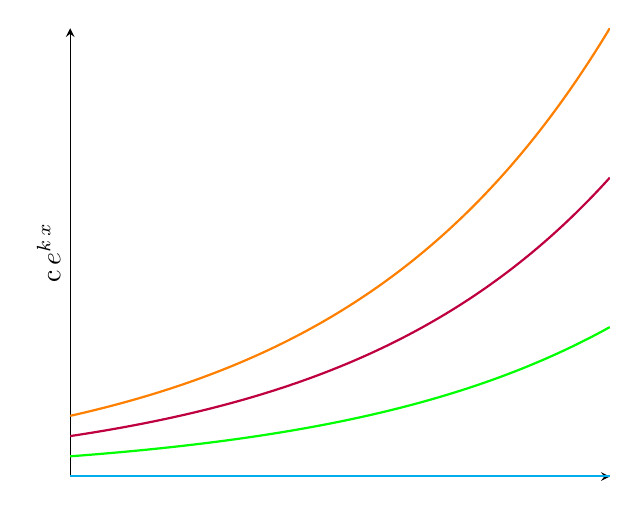
\begin{tikzpicture}
    \begin{axis}[
        axis x line = bottom,
        axis y line = left,
        ylabel = {$\mathrm{c} \, e^{k \, x}$},
        ticks = none
    ]
        \addplot[
            domain = 2:4,
            samples = 100,
            color = cyan,
            thick
        ]
        {0};

        \addplot[
            domain = 2:4,
            samples = 100,
            color = green,
            thick
        ]
        {e^x};

        \addplot[
            domain = 2:4,
            samples = 100,
            color = purple,
            thick
        ]
        {2 * e^x};

        \addplot[
            domain = 2:4,
            samples = 100,
            color = orange,
            thick
        ]
        {3 * e^x};
    \end{axis}
\end{tikzpicture}

            \end{minipage}
            \hfill
            \begin{minipage}[t]{.45\textwidth}
                \subsubsection*{Fissato \(k < 0\)}

                    %! TEX root = ../../../analisi2.tex

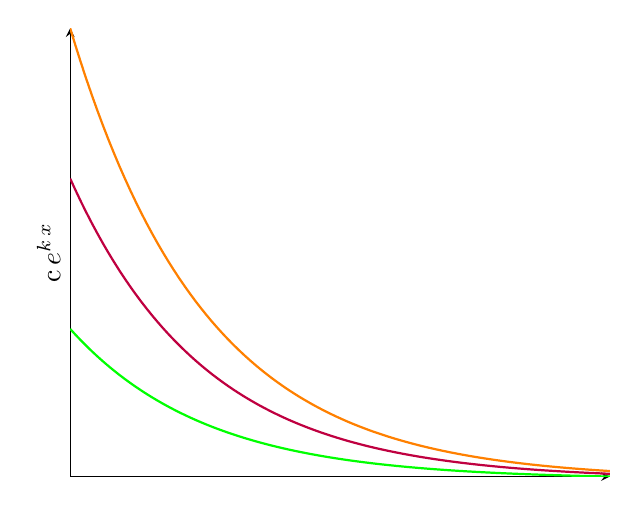
\begin{tikzpicture}
    \begin{axis}[
        axis x line = bottom,
        axis y line = left,
        ylabel = {$\mathrm{c} \, e^{k \, x}$},
        ticks = none
    ]

        \addplot[
            domain = 0:4,
            samples = 100,
            color = green,
            thick
        ]
        {e^(-x)};

        \addplot[
            domain = 0:4,
            samples = 100,
            color = purple,
            thick
        ]
        {2 * e^(-x)};

        \addplot[
            domain = 0:4,
            samples = 100,
            color = orange,
            thick
        ]
        {3 * e^(-x)};
    \end{axis}
\end{tikzpicture}

            \end{minipage}

            \medskip

            Riassumendo, questo modello prevede tre comportamenti possibili, in base a \(k\):
            \begin{itemize}
                \item Se \(k > 0\), cioè la natalità è superiore alla mortalità, la popolazione aumenta esponenzialmente;
                \item Se \(k = 0\), cioè la natalità è equivalente alla mortalità, la popolazione resta costante;
                \item Se \(k < 0\), cioè la natalità è inferiore alla mortalità, la popolazione si estingue esponenzialmente.
            \end{itemize}

        \section{Equazione logistica}

            L'equazione logistica è stata introdotta dal matematico francese Pierre François Verhulst verso la metà del 1800. Questa è più
            articolata rispetto alla precedente.

            La formulazione è la seguente: al crescere della popolazione, diventa più difficile procurarsi il cibo. Possiamo dunque
            definire un'equazione
            \[
                y'(x) = k \, y(x) - g(y(x)),
            \]
            con \(g\) funzione opportuna. una buona scelta di \(g\) risulta
            \[
                g(s) = h \, s^2,
            \]
            con \(h\) costante positiva. Dunque, l'equazione logistica diventa
            \[
                y'(x) = k \, y(x) - h \, y^2(x).
            \]

            \newpage

            Si tratta di un'equazione di Bernoulli con soluzioni:
            \begin{itemize}
                \item Soluzioni costanti:
                    \begin{align*}
                        y &= 0,\\
                        y &= \frac{k}{h};
                    \end{align*}
                \item Soluzioni non costanti:
                    \[
                        y(x) = \frac{k \, e^{k \, x}}{\mathrm{c} + h \, e^{k \, x}},
                    \]
                    dove \(x > 0\) e \(\mathrm{c} \in \R\) e con
                    \[
                        y(0) = \frac{k}{\mathrm{c} + h}.
                    \]
            \end{itemize}

            Studiamo graficamente l'andamento:

            \medskip

            \begin{center}
                %! TEX root = ../../../analisi2.tex

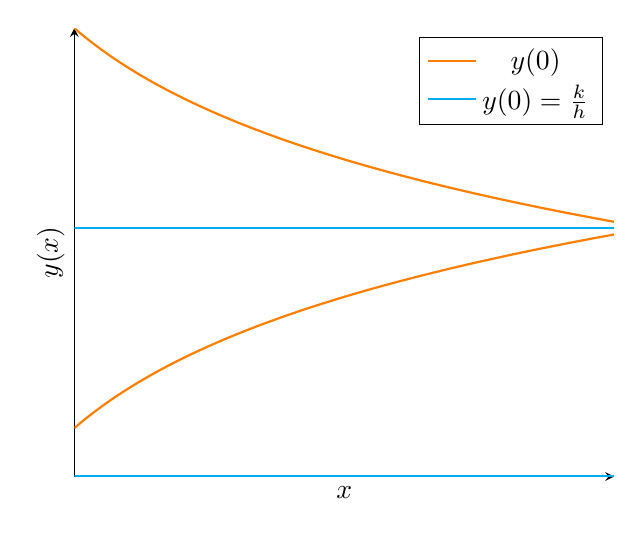
\begin{tikzpicture}
    \begin{axis}[
        axis x line = bottom,
        axis y line = left,
        ylabel = {$y(x)$},
        xlabel = {$x$},
        ticks = none
    ]

        \addplot[
            domain = .2:0.95,
            samples = 100,
            color = orange,
            thick
        ]
        {ln(x) + 2};
        \addlegendentry{$y(0)$}

        \addplot[
            domain = .2:0.95,
            samples = 100,
            color = cyan,
            thick
        ]
        {2};
        \addlegendentry{$y(0) = \frac{k}{h}$}
            
        \addplot[
            domain = .2:0.95,
            samples = 100,
            color = orange,
            thick
        ]
        {2 - ln(x)};

        \addplot[
            domain = .2:0.95,
            samples = 100,
            color = cyan,
            thick
        ]
        {0};
    \end{axis}
\end{tikzpicture}
            \end{center}

\end{document}